\documentclass[12pt,a4paper]{article}
\usepackage[spanish]{babel}
\usepackage[utf8]{inputenc}
\usepackage{graphicx}
\usepackage{graphics}
\usepackage{epsfig}
\usepackage{amsmath}
\usepackage{caption}
\usepackage{algorithm}
\usepackage{algorithmic}
\usepackage{url,hyperref,times}
\usepackage[T1]{fontenc}
\usepackage{color,listings,tikz}
\selectlanguage{spanish}
\usepackage{times}
\usepackage{verbatim,scalefnt,colortbl}
\newtheorem{mydef}{Definición}
\providecommand{\e}[1]{\ensuremath{\times 10^{#1}}}
\DeclareCaptionType{myeq}[][Lista de ecuaciones]
\captionsetup[myeq]{labelformat=empty}

\title{ {\bf Whole genome alignment in high performance computing environments} \\
\it Informe del progreso de trabajo de investigaci\'on} 
\author{ {\bf Julio C\'esar Garc\'ia Vizca\'ino}  \\ 
Departamento de Arquitectura de Computadores y Sistemas Operativos \\ 
Universidad Aut\'onoma de Barcelona\\ 
{\small jcgarcia@aomail.uab.es} 
}
\date{\today}

\begin{document}
\pagestyle{plain}
\pagenumbering{roman}
\maketitle
\pagebreak
{\Huge{\bf Datos del doctorando}}\\
{\Large \\Nombre Completo: Julio César García Vizcaíno\\}
\vspace{0.3cm}
{\Large NIE: Y1497678R\\}
{\Huge{\bf Datos del proyecto de tesis}}\\
\vspace{0.3cm}
{\Large \\Estudio de doctorado: Computación de Altas Prestaciones\\}
\vspace{0.3cm}
{\Large \\Título del proyecto de tesis doctoral: \emph{
Whole genome alignment in high performance computing environments.}\\}
\vspace{0.3cm}
%{\Large \\Palabras claves: Alineamiento de genoma, cadena coincidente,
%datos de secuencia biol\'ogica a gran escala, C\'omputo de altas prestaciones.\\}
%\vspace{0.5cm}
{\Large \\Directores de la tesis: Antonio Espinosa, Juan Carlos Moure.\\}
\vspace{0.3cm}
{\Large \\Línea de investigación: Aplicaciones bioinformáticas.\\}
\vspace{0.3cm}
{\Large \\Rgimen de dedicación: completa.\\}
\vspace{0.3cm}
{\Large \\A\~no de inscripci\'on: 2011.\\}
\vspace{0.3cm}
{\Large \\A\~no previsto para la presentaci\'on de Tesis Doctoral: 2014\\}
\vspace{0.3cm}
{\large \\Firmado\\}
\vspace{2.8cm}
\begin{center}
\begin{tabular}{ c c c }
Director & Director & Estudiante\\
Antonio Espinosa & Juan Carlos Moure & Julio C\'esar García Vizcaíno\\
\end{tabular}
\end{center}
\pagebreak
%\cleardoublepage
\pagenumbering{arabic}
\section{Resumen}
\indent
Actualmente la generación de nueva información genómica ha creado la necesidad de almacenar y procesar estos nuevos datos computacionalmente hablando. Una de las tareas en la que nos centramos es el alineamiento de genomas ya que es una tarea computacionalmente intensiva. La información básica de un genoma es el ADN. El ADN es una cadena compuesta por el alfabeto $\sigma={a,c,g,t}$, cada uno de estos elementos es llamado nucleótido. El alineamiento de genomas consiste en encontrar un mapeo de cada posición en un genoma de consulta a su correspondiente posición en el genoma de referencia. Es decir, encontrar las similitudes y diferencias de las cadenas de ADN entre genomas.\\
El alineamiento de genomas es un modelo matemático utilizado por los biólogos para determinar la similitud entre genomas. 
%Un alineamiento involucra tres operaciones básicas:
%\begin{itemize}
%  \item Coincidencia: los nucleótido en ambos genomas son iguales.
%  \item Discrepancia: los nucleótidos no coinciden en ambos genomas.
%  \item Mutaciones: uno o varios cambios de nucleótidos en el genoma:
%    \begin{itemize}
%      \item Sustitución: un nucleótido es reemplazado por otro.
%      \item Inserción: uno o varios nucleótidos se insertan en una posición en el genoma.
%      \item Eliminación: uno o varios nucleótidos se borran del genoma.
%    \end{itemize}
%\end{itemize}
%Los algoritmos utilizados para el alineamiento de genomas presentan una alta demanda computacional debido al tamaño de los datos genómicos.\\
\indent
Existe diferentes algoritmos propuestos para el alineamiento de dos secuencias como \cite{Needleman1970General} y \cite{Waterman}. Estos algoritmos funcionan bien con tamaños de secuencias pequeños como un gen, 20-30kbp\footnote{bp es la únidad básica de medida en las secuencias de ADN y representa la longitud de un nucleótido}. Sin embargo, son ineficaces al alinear genomas enteros. La complejidad computacional y espacial es $O(nm)$, donde $n$ y $m$ son las longitudes de los genomas a alinear. Estos algoritmos tienen problemas de mayores requerimientos de memoria o de tiempos de ejecución inaceptables.\\
\indent
Para grandes secuencias, como el genoma humano (3Gbp), el uso de recursos computacionales pueden ser extremadamente grande y con un largo tiempo de ejecución. Es por ello que han surgido alternativas para reducir el tiempo de ejecución del alineamiento de secuencias. Una de esas alternativas es la utilización de la heurística basada en las coincidencias exactas máximas en las secuencias a alinear. Al encontrar las coincidencias máximas  únicas se puede realizar el alineamiento de genomas enteros reduciendo el espacio del alineamiento a las regiones entre las coincidencias máximas únicas.\\
\indent
Formalmente el problema de la búsqueda de coincidencias máximas únicas se define como:
\begin{mydef}
  Dadas dos secuencias (genomas) $R=r_{1}r_{2}\hdots r_{n}$ y $Q=q_{1}q_{2}\hdots q_{m}$, y una longitud mínima $l$, se requiere encontrar todas las ocurrencias de las coincidencias máximas únicas de longitud mínima $l$, entre $R$ y $Q$.
\end{mydef}
Existen diferentes aproximaciones para resolver el problema ver Figura \ref{fig:state}, todas ellas involucran un uso intensivo de recursos de cómputo (memoria, procesador).
\begin{figure}[h] 
   \centering 
   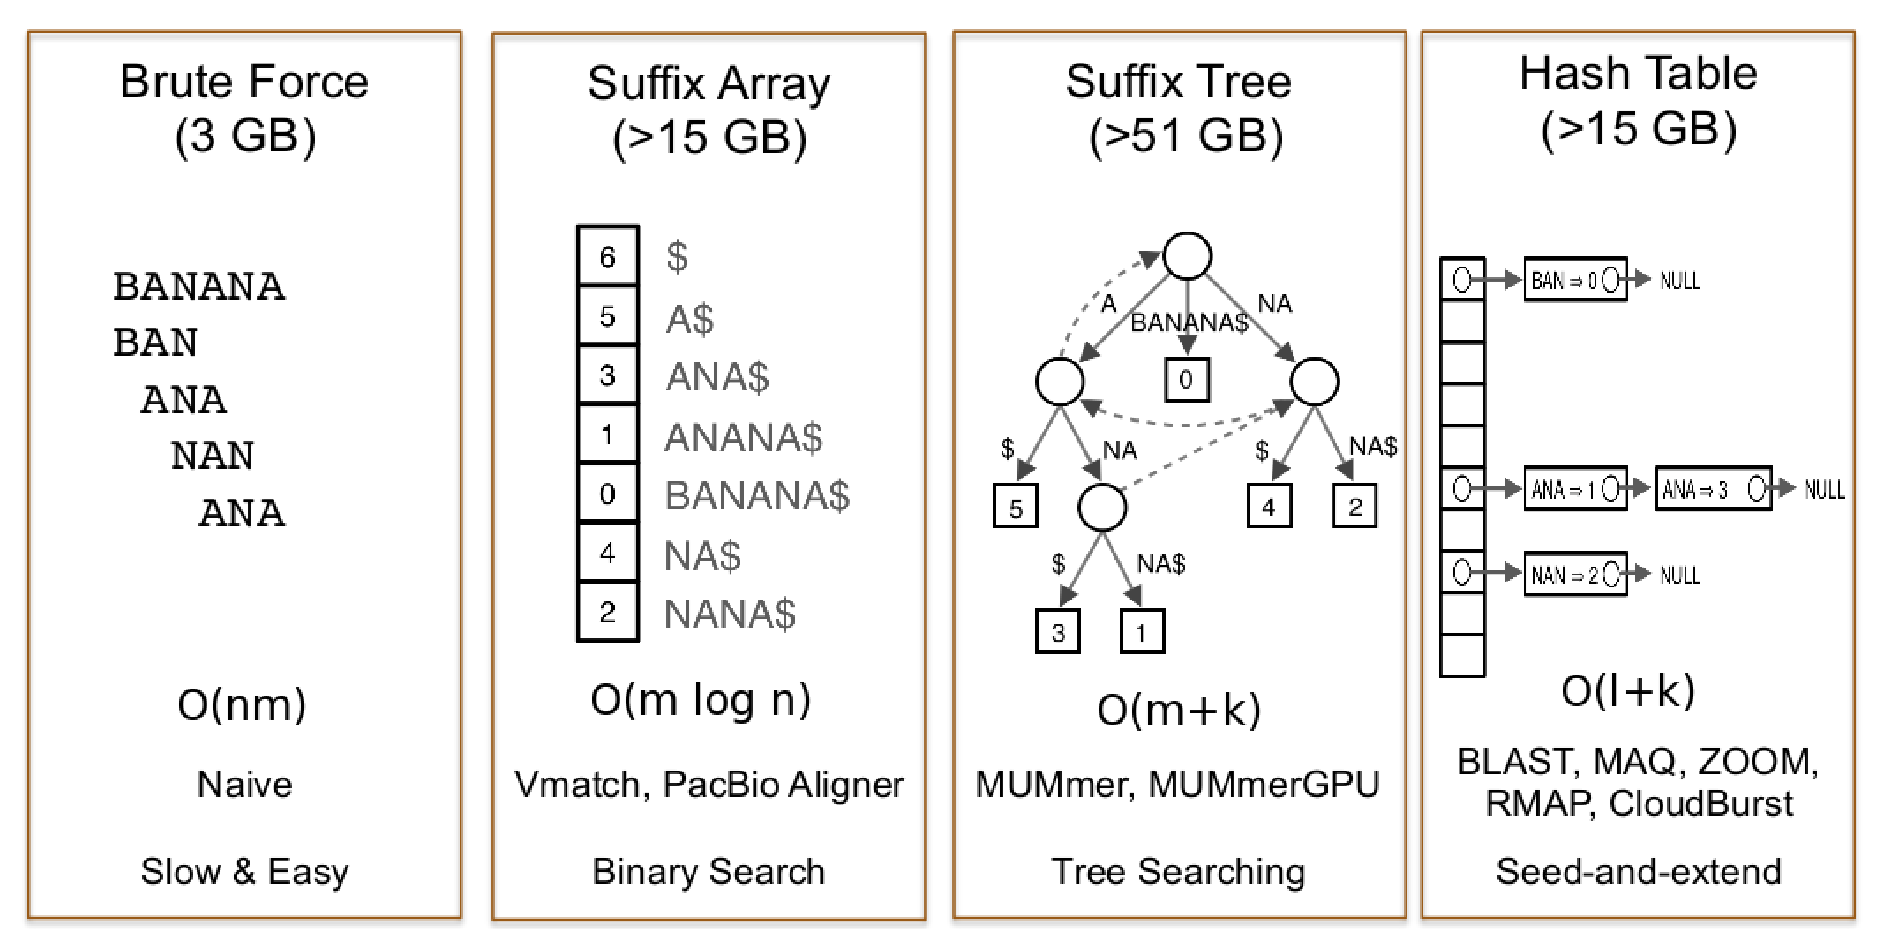
\includegraphics[scale=0.3]{state.eps} 
   \caption{Diferentes estructuras de indexación para el problema de la búsqueda de coincidencias exactas máximas para el genoma humano como referencia.} 
   \label{fig:state} 
 \end{figure}
\indent
%El árbol de sufijos es una estructura de datos que permite la b\'usqueda de coincidencias exactas de longitud variable en tiempo lineal respecto a la longitud de la secuencia de consulta. Una coincidencia exacta de longitud $w$ ocurre en $r_{i}r_{i+1}\hdots r_{i+l-1}$ y $q_{j}q_{j+1}\hdots q_{j+l-1}$ si y solo si los sufijos $r_{i}r_{i+1}\hdots r_{n}$ y $q_{j}q_{j+1}\hdots q_{m}$ comparten un prefijo común de longitud mínima $l$. La búsqueda de coincidencias máximas exactas en un árbol de sufijos se realiza recorriendo el trayecto que es común a la secuencia de consulta hasta encontrar una discrepancia. Si la búsqueda termina en un nodo hoja, la coincidencia es única en la secuencia de referencia. Verificando el carácter inmediato anterior al inicio de esta coincidencia se puede determinar si es una coincidencia máxima.\\
%\indent
%Este problema se presenta en aplicaciones de alineamiento de genomas donde el tama\~no de los genomas son de millones de caracteres y en consecuencia la búsqueda de MUMs es una tarea computacionalmente intensiva. Además, la razón de utilizar un árbol de sufijos radica en que la búsqueda de coincidencias exactas de longitud variable en un árbol de 
%sufijos se realiza en tiempo lineal, gracias al uso de los enlaces de sufijos.\\
%\indent
En consecuencia se busca \textbf{acelerar la búsqueda eficiente de 
coincidencias máximas únicas y que tenga en cuenta el uso de recursos de cómputo y
memoria en un clúster multicore}. Las consideraciones que se toman en cuenta son:
\begin{itemize}
\item Reducir el número de operaciones en la búsqueda de MUMs: al agilizar la búsqueda se reduce el tiempo utilizado por cada MUM encontrado.
\item Almacenar genomas de mayor tamaño con la memoria disponible: se hace necesario diseñar estructuras de datos que permitan la indexación de genomas mayores con menor uso de memoria, manteniendo la funcionalidad de la búsqueda de MUMS.
\item Mejorar la localidad de los datos para reducir los fallos en cache y garantizar un menor tiempo de ejecución.\end{itemize}
\section{Introducción} 
\subsection{MUM y MEM} 
\indent
La heurística basada en la búsqueda de coincidencias exactas máximas para el alineamiento de genomas requiere de la definición formal de una coincidencia exacta máxima (MEM).\\
\begin{mydef}
  Un MEM (Maximal Exact Match) es una subcadena común a dos
  genomas que es mayor que una longitud mínima específica $d$ de tal manera
  que es máxima, esto es, que no puede ser extendida en ambos extremos sin
  incurrir en una discrepancia. 
\end{mydef}
\indent
Adicionalmente, a partir de la definición de MEM surge el concepto de la coincidencia única máxima (MUM).\\
\begin{mydef}Un MUM (Maximal Unique Match) es una subcadena única común a dos genomas que es mayor que una longitud mínima específica $d$ de tal manera que es máxima, esto es, que no puede ser extendida en ambos extremos sin incurrir en una discrepancia.
\end{mydef}
Identificar las cadenas, $k$, mas grandes en el genoma $Q$ que tienen una coincidencia de longitud $l$ idéntica en el genoma $R$, tiene la siguiente complejidad computacional:
\begin{itemize}
  \item Método simple: $O(nl)$
  \item Usando árbol de sufijos: $O(l+k)$
\end{itemize}
\indent
El objetivo es buscar todas aquellas subcadenas que son comunes a las secuencias de referencia $R$ y consulta $Q$ que son máximas de longitud.\\
\subsection{Árbol de sufijos}
\indent
 Cualquier cadena de referencia de longitud $n$ puede ser descompuesta en $s$ sufijos, ver
 Figura \ref{fig:st}, y estos sufijos pueden almacenarse en un árbol de sufijos.
 Para crear esta estructura de datos se requiere de un tiempo $O(n)$ y para
 buscar una cadena en él requiere de un tiempo $O(l)$ donde $l$ es la longitud
 de la cadena \cite{Gusfield2007Algorithms}. Estas dos propiedades hacen al árbol
 de sufijos una estructura útil para un rango diverso de aplicaciones
 bioinformáticas, incluyendo: alineamiento de genomas \cite{Mummer3}.\\
   \begin{figure}[h] 
   \centering 
   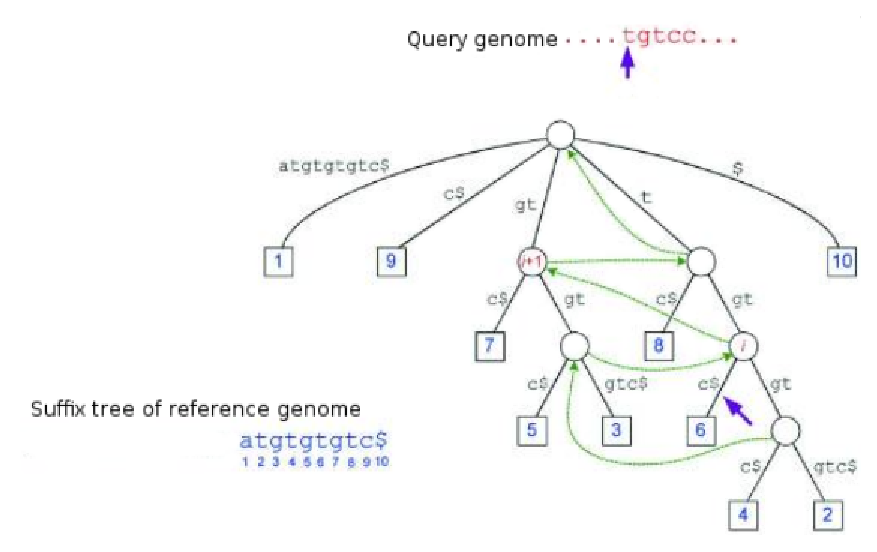
\includegraphics[scale=0.8]{st-mum.eps} 
   \caption{Árbol de sufijos para la palabra atgtgtgtc\$.} 
   \label{fig:st} 
 \end{figure}
\indent
La búsqueda de coincidencias exactas máximas en un árbol de sufijos se realiza recorriendo el árbol
con la cadena que se requiere encontrar la coincidencia exacta máxima. Si la coincidencia termina en 
un nodo hoja, la coincidencia exacta máxima es única en la secuencia de referencia. Verificando el 
carácter inmediato anterior al inicio de la posición de la coincidencia es posible determinar si es
máxima.\\
\indent
Por lo tanto es posible identificar todas las coincidencias exactas máximas en tiempo proporcional a
la longitud del genoma de consulta. Es importante resaltar que las coincidencias encontradas no son
necesariamente únicas en el genoma de consulta. Esto se debe a que al recorrer el genoma de consulta, 
las coincidencias encontradas no nos permiten identificar si son únicas ya que no es posible determinar
que coincidencias se encontrarán posteriormente en el genoma de consulta.\\
\indent
En la Figura \ref{fig:st} se muestra como una secuencia de consulta es buscada en el árbol de sufijos. El
árbol representa la secuencia de referencia atgtgtgtc\$. Las hojas representadas en la figura \ref{fig:st} por cuadrados indican la
posición en la que inicia el sufijo. Por ejemplo, la hoja 7 representa el sufijo gtc\$ que inicia en la 
posición 7 de la secuencia de referencia y que está formado por la secuencia de aristas etiquetadas desde la
raíz hasta el nodo hoja 7. En el punto mostrado en la figura, se ha encontrado la coincidencia en la posición $i$,
indicada por la flecha. La coincidencia se extiende a la correspondiente posición en el árbol. En este caso sabemos
que la coincidencia es única en la referencia por que estamos ubicados en un nodo hoja. El número del nodo hoja
nos da la posición de inicio de la coincidencia en la referencia.\\
\indent
Para encontrar la siguiente coincidencia en la cadena de consulta, usamos los enlaces de sufijos, señalados en la Figura \ref{fig:st} por
flechas punteadas. Estos enlaces son construidos para cada nodo interno en el árbol. Un enlace apunta de un nodo
$x$ a un nodo $y$ si el sufijo de la raíz a $y$ es igual al sufijo desde la raíz a $x$ con el primer carácter 
eliminado. Por ejemplo, la cadena del nodo $i$ en la Figura \ref{fig:st} es tgt y del nodo $i+1$ es gt. Esa es la
posición en el árbol correspondiente a la siguiente posición en la secuencia de consulta. Desde el nodo $i$ podemos
continuar la coincidencia bajando en el árbol para determinar que tan grande es la coincidencia puede extenderse. Las 
coincidencias son máximas hacia la derecha cuando se buscan en el árbol de sufijos. Para verificar si son máximas a
la izquierda comparamos los caracteres precedentes en cada cadena. En el ejemplo de la Figura \ref{fig:st}, la
coincidencia inicia en $i+1$ en la cadena de consulta y en el nodo 7 de la cadena del árbol no es máxima a la izquierda
porque el carácter precedente en ambas cadenas es $t$.\\
\indent
La clave para la búsqueda veloz en un árbol de sufijos es que 
hay un camino desde la raíz para cada sufijo del texto. Esto significa que se 
necesitan $l$ comparaciones para encontrar una cadena de longitud $l$.\\
\indent
Otra mejora de implementación necesario para conseguir un tiempo y espacio 
lineal es el uso de enlaces de sufijos. Un enlace de sufijo es un puntero de un 
nodo interno etiquetado $xS$ a otro nodo interno etiquetado $S$, donde $x$ es un 
carácter arbitrario y $S$ es posiblemente una subcadena vacía. Los enlaces de 
sufijos permiten agilizar el recorrido del árbol sin visitar la raíz del árbol 
debido a que apuntan a la siguiente extensión del sufijo. Los enlaces de sufijos 
y la compresión de las etiquetas de las aristas son los requerimientos claves 
para la implementación del árbol de sufijos en $O(n)$.\\
\subsection{Definición del problema a resolver}
\indent
El problema de la búsqueda de las coincidencias máximas únicas de una longitud mínima ha sido identificado en varias aplicaciones, entre ellas MUMmer \cite{Mummer3}. Aunque el algoritmo de MUMmer realiza la búsqueda de coincidencias exactas máximas, los requerimientos de recursos de cómputo aún son altos debido al tamaño de los datos de entrada.\\
\indent
Si la longitud de los genomas son muy grandes, ver Cuadro \ref{tab:buscar3}, 
la cantidad de búsquedas aumentan, el tiempo de búsqueda
crece linealmente y el uso de memoria se convierte en un problema a resolver si
se considera la disponibilidad finita de memoria en la mayoría de sistemas de
cómputo personales.\\
\begin{table}[ h!]
  \begin{small}
    \begin{center}
      \begin{tabular}{lllll}
        Estructura & L [bp\footnote{Par base, unidad básica de medición de nucleótidos en una secuencia de ADN.}] & Cantidad  & Búsqueda [s] & Uso de\\
        & & de búsquedas & & memoria [MB]\\
        \hline
        Árbol de sufijos & 20 & 9,87\e{18}  & 169189,4 & 48665,12\\
        \hline
        %Arreglo de sufijos & 20 & 9,87\e{18}  & 593019,3 & 32241,9\\
        %\hline
      \end{tabular}
    \end{center}
  \end{small}
  \caption{Búsqueda coincidencias exactas para una cadena de referencia de 
  2960,21Mbp y una cadena de consulta de 2716,96Mbp}
  \label{tab:buscar3}
\end{table}
\indent
De acuerdo a los datos del Cuadrs \ref{tab:buscar3} se hace necesario la búsqueda de alternativas que 
permitan llevar a cabo la búsqueda de manera eficiente. El uso de HPC nos permitiría
resolver los problemas de escalabilidad (tiempo de búsqueda, uso de memoria) cuando 
se tienen cadenas muy grandes, como el genoma humano.\\
En consecuencia, para resolver este problema se utiliza alguna estructura de datos que 
permita realizar una búsqueda distribuida de coincidencias máximas únicas de forma ágil 
en el genoma entero. 
\indent
En resumen la búsqueda de coincidencias exactas máximas en una cadena, como el 
genoma humano, es un problema computacionalmente intensivo que es posible 
resolverse con estructuras de datos de indexación de cadenas. 
\indent
Independientemente de la estructura de datos utilizada, lo que se desea es poder realizar búsquedas de coincidencias exactas a esa estructura de manera eficiente. 
Una de las consultas en que se requiere realizar rápidamente, para el alineamiento de genomas, es la búsqueda de coincidencias máximas únicas. 
\section{Estado de la investigación}
La búsqueda de MUMS entre un genoma de Referencia y uno de Consulta tiene una característica importante que puede ayudarnos a paralizar su búsqueda: podemos buscar más de un sufijo a la vez del genoma de Consulta. Utilizando una estructura de datos de indexación para buscar MUMs, encontramos MUM candidatos al ir recorriendo el genoma de Consulta. Un MUM candidato es un MUM que se almacena como un posible MUM pero que se tiene que verificar al final de la fase de búsqueda para garantizar que es un MUM único en el genoma de Consulta.
El estado actual de la investigación consiste en la evaluación de la estructura de datos (árbol de sufijos) utilizada en el algoritmo actual de la aplicación MUMmer, determinar los problemas de rendimiento entre el algoritmo y la estructura de datos y finalmente estudiar, evaluar y modificar la estructura de datos (Arreglo de sufijos mejorado) que permite reducir el tiempo de ejecución, mejor localidad espacial y temporal y la reducción en el uso de memoria.
Finalmente se ha realizado una paralelización de la búsqueda de MUMs mediante OpenMP para su utilización en arquitecturas multi-core con el árbol de sufijos y con el arreglo de sufijos mejorado.
Todos los experimentos se han desarrollado en el siguiente entorno:
\begin{enumerate}
\item GCC 4.7 con OpenMP + Linux
\item MUMmer 3.23
\item 2 procesadores Intel(R) Core(TM)2 Duo CPU     E8400  @ 3.00GHz, con 6 cores cada procesador: 32KB cache L1 por core, 256KB cache L2 por core y 12MB cache L3 compartida.
\item RAM 96GB
\end{enumerate}
\subsection{Problemas de rendimiento en el árbol de sufijos}
La búsqueda de MUMs mediante un árbol de sufijos tiene una complejidad lineal debido al uso de los enlaces de sufijos. El enlace de sufijo permite saltar a otra posición del árbol de sufijos con el siguiente sufijo evitando la necesidad de recorrer el árbol de sufijos desde el inicio del sufijo. 
Sin embargo el árbol de sufijos sufre de un problema de localidad espacial y temporal. Lo que convierte a la estructura en el cuello de botella del rendimiento del algoritmo de búsqueda de MUMs.
Para demostrar que el árbol de sufijos sufre de problemas de localidad espacial y temporal se ha realizado una evaluación experimental para determinar el efecto de mantener un árbol de sufijos en el último nivel de cache y mantener el árbol de sufijos en memoria principal.
\subsubsection{Evaluación experimental}
\indent
Al mantener la estructura de datos en cache la búsqueda de MUMs será más rápida. Al crecer la estructura de datos se debe mantener en memoria principal, lo que ocasiona una disminución en las prestaciones del algoritmo de búsqueda de MUMs.
Para demostrar la falta de localidad espacial del árbol de sufijos se estudiaron dos escenarios:
\begin{enumerate}
\item Árbol de sufijos cabe en el último nivel de cache.
\item Árbol de sufijos cabe en memoria principal.
\end{enumerate}
Los genomas de Referencia utilizados fueron de 312Kbp y 170Mbp, el genoma de Consulta fue de 169Mbp en todos los experimentos. Al mantener la longitud del genoma de consulta constante garantizamos mantener la complejidad de la búsqueda de MUMs.
El primer parámetro medido fue el CPI, al tener el árbol de sufijos en cache el CPI es de 1.61 y al tener el árbol de sufijos en memoria principal el CPI aumenta a 4.98, 3 veces mas que mantener el árbol de sufijos en cache. La razón de este aumento es el crecimiento de los ciclos de reloj en el segundo escenario, ya que las instrucciones ejecutadas prácticamente es el mismo en ambos escenarios.
Respecto a los fallos de cache por instrucción, en L1 aumentan 12\% con respecto al escenario 1, en L2 23.79\% y en L3 los fallos pasan de 0.01\% a 2.83\%. Eso nos demuestra que la falta de localidad espacial del árbol de sufijos es relevante cuando el genoma de referencia indexado no se puede almacenar en algún nivel de cache. Las instrucciones de Load y Store se mantienen prácticamente igual. Adicionalmente el ancho de banda en la jerarquía de memoria es mayor en cache 2 y 3 en el escenario 1; en el escenario 2 el ancho de banda es mayor en memoria principal, pero en cache 2 cae un 64\% y en cache 3 cae un 65\% con respecto al escenario 1.
\subsection{Paralelización de búsqueda de MUMs en Árbol de sufijos}
Debido a los problemas de localidad espacial del árbol de sufijos se elaboró una propuesta de paralización
\indent
Los genomas utilizados en las pruebas fueron:
\begin{itemize}
\item Genoma humano (2,96Gbp).
\item Cromosoma 2 humano (238,6Mbp).
\item Cromosoma 1 chimpancé (232,7Mbp).
\item EcoliK12 (4,6Mbp).
\item EcoliO157H7 (5,3Mbp).
\end{itemize}

\section{Publicaciones}
\noindent
Ninguna.
\section{Seguimiento}
En el primer año se ha cumplido con la adaptación de una estructura de datos que permita su utilización
en el alineamiento de datos biológicos a gran escala. Dicha estructura será la base del desarrollo de MUMmer en HPC.
La estructura es capaz de manejar grandes volúmenes de datos y se pueden realizar operaciones de consulta sobre ella.
\section{Planificación}
En el segundo año se realizará el diseño y evaluación experimental de un algoritmo paralelo y distribuido de búsquedas de 
coincidencias exactas máximas. Para ello se aprovechará la estructura de datos diseñada en el primer año. Se adaptará este
algoritmo a la aplicación MUMmer para su ejecución en entornos de HPC.
En el tercer año se refinará la ejecución de MUMmer en entornos de HPC. Se tomará como base el programa original, MUMmer, y 
se realizarán las modificaciones pertinentes para mejorar la fase de agrupamientos de MUMs y MEMs. Estancia en otra unidad 
de investigación, EMBL Heidelberg Alemania. Adaptar la propuesta de búsqueda distribuida de coincidencias exactas desarrollado para su
ejecución en las instalaciones de EMBL. Redactar la tesis doctoral y preparar su defensa.
\section{Análisis de las publicaciones pendientes de publicar}
\noindent
Ninguna.
\section{Publicaciones previstas}
%Asia Pacific Bioinformatics Conference - \href{http://www.apbc2013.org/}{APBC} - Julio 2012 : Una tema de investigación en el congreso es Comparative genomics que forma parte del problema que se está resolviendo, el alineamiento de genomas.\\
IEEE International Symposium on Parallel and Distributed Processing with Applications - \href{http://www.arcos.inf.uc3m.es/ispa12/}{ISPA} - Enero 2013 : La estructura del árbol de sufijos distribuidos forma parte de los temas de investigación en este congreso.\\
International Conference on Parallel Processing - \href{http://www.grs-sim.de/news-events/news-archive/euro-par-2013.html}{Euro-Par} - Febrero 2013 : El algoritmo de búsqueda de coincidencias exactas máximas distribuida forma parte de los temas aboradados en este congreso.\\
European Symposium on Algorithms - \href{http://esa-symposium.org/}{ESA} - Abril 2013 : El algoritmo de búsqueda distribuida de coincidencias exactas máximas distribuida forma parte de los temas abordados en este congreso.\\
International Symposium on Algorithms and Computation - \href{http://www.is.titech.ac.jp/isaac11/}{ISAAC} - Junio 2013 :  El algoritmo de búsqueda distribuida de coincidencias exactas máximas distribuida forma parte de los temas abordados en este congreso.\\
\section{Conclusiones}
\indent
Durante este primer año de investigación doctoral se ha estudiado y evaluado la estructura de datos utilizada en la aplicación MUMMer.
Se ha mejorado la fase de obtención de la lista final de MEMs reduciendo la complejidad del algoritmo utilizado previamente.
Se han diseñado diferentes experimentos para determinar la mejor manera de dividir dicha estructura y aprovechar la nueva estructura
en entornos de HPC. Se evalúo la utilidad de los enlaces de sufijos en un árbol de sufijos y como se pueden aprovechar para la 
búsqueda de coincidencias exactas máximas.\\
\indent
Se ha adaptado el árbol de sufijos para su ejecución en entornos de HPC y se ha propuesto una solución al problema de  la restricción
de memoria cuando la cadena de referencia crece. La estructura de datos adaptada se ha utilizado para proponer una primera aproximación a la 
solución de mejorar el tiempo de búsqueda de coincidencias exactas máximas.\\
\indent
En el siguiente año se busca determinar si la propuesta de búsqueda de coincidencias exactas máximas en el árbol de sufijos distribuido 
permite mejorar el tiempo de ejecución bajo entornos de HPC. Adicionalmente se tendrán que resolver los siguientes problemas
\begin{itemize}
  \item Política de carga de trabajo para cada árbol de sufijos disperso: garantizar que todas las búsquedas se resuelvan de manera local.
  \item Búsqueda de coincidencias exactas máximas en el árbol de sufijos disperso de forma paralela, es decir, realizar múltiples búsquedas
    para distintos sufijos bajo el paradigma de las arquitecturas multicore. 
\end{itemize}
\bibliographystyle{apalike} 
\bibliography{references}	
\end{document}
